Vier quaderförmige Körper werden auf eine ihrer unteren Kanten gekippt und in dieser Lage losgelassen. Ihre Grundfläche ist dann um den Winkel $\theta$ gegen den Boden geneigt. A und D sind unten beschwert, ihr Schwerpunkt S liegt deshalb tiefer als die Mitte; B und C sind homogen. $h_\mathrm{S}$ ist die Höhe von S über der Grundfläche.
\begin{center}
\begin{tabular}{lcccc}
 Körper & A & B & C & D \\ \hline
 Breite $b$ & \wAO & \wBO & \wCO & \wDO \\
 Höhe $h$ & \hAO & \hBO & \hCO & \hDO \\
 Schwerpunkthöhe $h_\mathrm{S}$ & \sAO & \sBO & \sCO & \sDO \\
 Neigung $\theta$ & \tAO & \tBO & \tCO & \tDO
\end{tabular}
\end{center}
\begin{center}
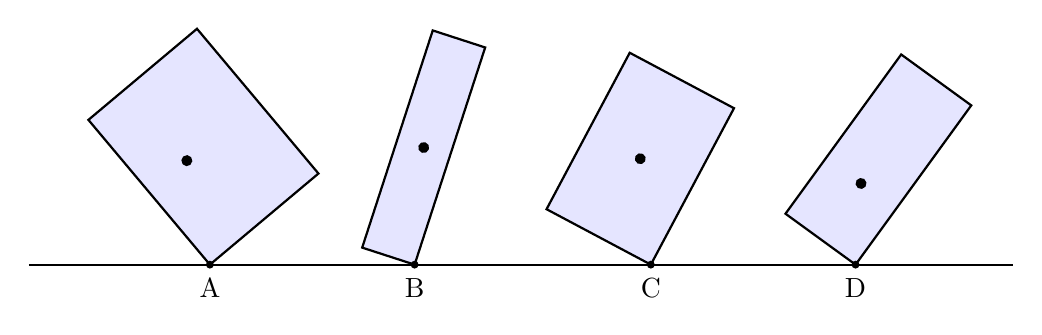
\begin{tikzpicture}[scale=1]
 \draw[thick] (-0.3,0) -- (12.2,0);
 \foreach \x/\w/\h/\s/\t/\n in {2/2.4/1.8/0.625/50/A, 4.6/0.7/2.9/1.45/18/B, 7.6/1.5/2.25/1.125/28/C, 10.2/1.1/2.5/0.875/36/D} {
  \begin{scope}[shift={(\x,0)}, rotate=-\t]
   \draw[thick, fill=blue!10] (-\w,0) rectangle (0,\h);
   \fill (-\w/2,\s) circle (0.07);
  \end{scope}
  \fill (\x,0) circle (0.05);
  \node[below] at (\x,-0.05) {\n};
 }
\end{tikzpicture}
\end{center}

\begin{abcliste}
\abc
\DuSie{Ordne}{Ordnen Sie} die Körper nach ihrer Neigung. Fällt der am stärksten geneigte Körper um?

\abc
Welche Körper fallen um, welche fallen auf ihre Grundfläche zurück? \DuSie{Begründe}{Begründen Sie} mit dem Schwerpunkt und \DuSie{rechne}{rechnen Sie} nach.
\end{abcliste}
